\chapter{Depth Estimation}
\label{sec:depthestimation_theory}


In this chapter we look at some of the core principals of depth
estimation theory, and some of the previous work done in the field.

\section{Introduction}

Extracting depth from images has been a heavily researched area of
computer vision for decades. As a result, there are many vastly
different techniques. But common for all the techniques are the

In short, depth estimation is about finding points in a 3D scene that
can be identified in two images taken from different points of
view. For each point, the difference in a points pixel coordinates in
one view relative to the other view, gives us the points disparity.

By finding the disparity of each point that is visible in both images,
we get a disparity map. With these disparity values, we can roughly
calculate the physical distance to these points from the cameras.

A simple demonstration of how two views viewing the same scene
changes; hold a finger vertically in front of your eyes. Close one of
your eyes alternatively, and notice how the fingers position changes
relative to the background. This change of position between the view
is the disparity. With some triangulation, the depth can be estimated.

\begin{figure}
  \label{fig:depth-theory}
  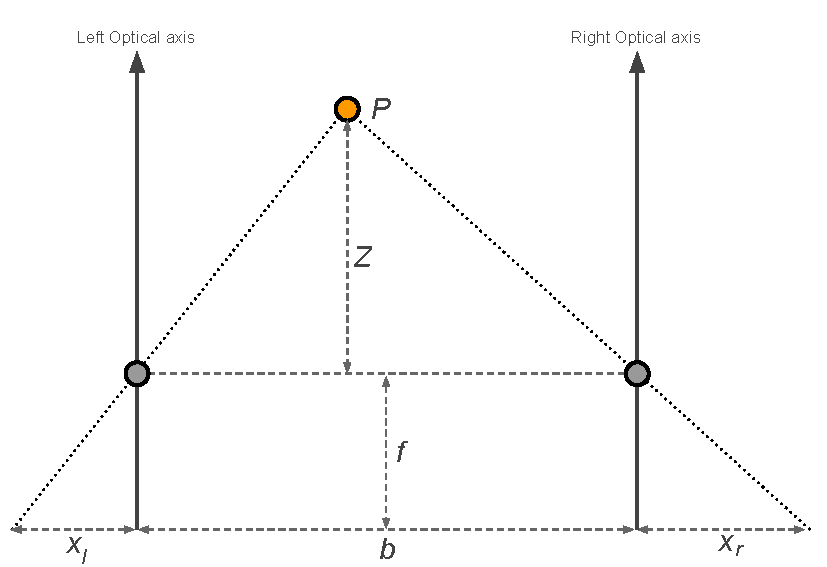
\includegraphics[width=\textwidth]{images/depth-estimation-theory.pdf}
  \caption{Example of how the depth can be calculated}
\end{figure}

Figure \ref{fig:depth-theory} shows how the depth \textit{Z} can be
triangulated. Finding the disparities \textit{Xl} and
\textit{Xr} is the main difficulty.


\section{Related Work}

Scharstein and Szeliski presents a very thorough taxonomy and
evaluation of some of the most known stereo correspondence algorithms
in \cite{taxonomy}. Most algorithms can be grouped into 3 distinct
sets:

\begin{itemize}
\item Feature-based
\item Graph cuts
\item Correlation based
\end{itemize}




\section{Depth Estimation Algorithms}

It is observed that most algorithms generally perform the following
four steps (or subsets of) \cite{taxonomy} :

\begin{enumerate}
\item Matching Cost computation
\item Cost (support) aggregation
\item Disparity computation/optimization
\item Disparity refinement
\end{enumerate}

Most stereo algorithms can be grouped into two main categories;
\textit{local} and \textit{global} algorithms.

Local algorithms estimate depth with the help of its neighboring
pixels only. This neighborhood varies between algorithms, but is most
often a square window of $7\times7$ to $21\times21$ pixels. Other
local algorithms may use adaptive windows that changes shape on
certain conditions, or non-square shapes.

Global algorithms make explicit smoothness assumptions and then solve
an optimization problem. This thesis will not cover global algorithms.

\subsection{Matching Cost calculation}
\label{sec:matchingcost}

The matching cost is a measurement of the similarity of pixel
locations in the input images. This calculation is typically done for
all pixels, at all the disparity hypotheses.

There are many ways to calculate this. Two of the simplest methods are
\textit{Absolute intensity differences} (AD) and \textit{Squared
  intensity differences} (SD). These methods are very computationally
quick to calculate, AD even more so than SD.


\begin{figure}
  \label{eq:sad}
  \[ \mathlarger{\mathlarger{\sum}}_{i,j \in w} |I_L(i,j) - I_R(x + i, y + j)| \]
  \caption{Sum of Absolute intensity Differences}
\end{figure}


\begin{figure}
  \label{eq:ssd}
  \[ \mathlarger{\mathlarger{\sum}}_{i,j \in w} (I_L(i,j) - I_R(x + i, y + j))^2 \]
  \caption{Sum of Squared intensity Differences}
\end{figure}

A third well known technique is \textit{Birchfield and Tomasi}'s (BT)
image sampling insensitive method \cite{bt}. Instead of comparing
pixel values shifted by integral amounts, BT compares each pixel in
the reference image against a linearly interpolated function of the
other image.

\begin{equation}
  \label{eq:bt}
  \mathlarger{\mathlarger{\sum}}_{i,j \in w} d(x_L, x_R, I_L, I_R) = \max\{0, I_L(x_L) - I_{max}, I_{min} - I_L(x_L) \}
\end{equation}


A lower cost is a better match, where a cost of 0 means the left and
right pixels are identical.

\subsection{Aggregation of Costs}
\label{sec:aggregatecost}

Single pixel matching is in most cases too ambiguous. Some kind of
additional information is needed. For \textit{local} algorithms,
summing or averaging a small neighborhood of pixel-costs into an
aggregated cost yields a much better value for comparison.

The simplest way is to sum the costs in a window around the pixel of
interest. This method is known as \textit{Sum of Absolute Differences}
(SAD) or \textit{Sum of Squared Differences}, depending on which cost
matching was used.

Another slightly more complex technique is to use \textit{Adaptive
  Windows}\cite{Okutomi and Kanade, 1992; Kanade and Okutomi, 1994;
  Veksler, 2001; Kang et al., 2001)}. Figure \ref{fig:adaptivewindow}
demonstrates what an adaptive window looks like. Cost matching is done
normally with either AD or SD. Each square is then aggregated
separately. What gives this technique its name is which of the squares
are used as the final aggregation cost; it selects the two windows
with the lowest scores, and the center square. This method is better
along depth disparities, since windows spanning an occlusion is much
less likely to be included in the final selection.

A lower aggregated cost is a better match, where a cost of 0 means the
left and right pixels and its neighborhood are identical.

\subsection{Disparity Selection}
\label{sec:disparity_selection}

This step involves finding which disparity level has the best
match. The easiest way is to compare each cost at each disparity
level, and select the level with the lowest cost. This strategy is
called \textit{winner-takes-all} (WTA).




\subsection{Refinement}
\label{sec:refinement}

Most depth estimation algorithms produce a disparity map of integer
disparities. Many applications such as robotics navigation and
tracking are fine with that level of quantization. However, for
image-based rendering such as \textit{Visual Hulls} and
3D-reconstruction, this level is detail is detrimental to the quality
of their output. This can be alleviated by applying a sub-pixel
refinement stage. Linear interpolation may be too simple, but others
have researched methods like including an iterative gradient descent
and fitting a curve to the matching costs at discrete disparity levels
\cite{Ryan et al., 1980; Lucas and Kanade, 1981; Tian and Huhns, 1986;
  Matthies et al., 1989; Kanade and okutomi, 1994, taxonomy}.

Applying a median filter to the disparity map removes high-intensity
noise caused by erroneous and spurious matches. Along an objects
surface the disparity is most likely going to be continuous, and
blurring may even out slightly-off matches.

Cross-checking is a method that requires a disparity map for both the
left and right images.

Cross-checking eliminates unreliable matches. All depth
discontinuities will have occlusions, where a real world point is only
visible on one of the images, and will also always produce an
unreliable match.

When cross-checking and eliminating unreliable matches, holes of
uncalculable disparity are left in the disparity map. These holes can
be artificially filled with guesses; it is very likely that the
disparity in the occlusions are continuous

sub-pixel refining

\section{Summary}

Depth estimation is about
